\section{Discussion: The Political Economy of Capacity Utilization in the Center and the Periphery}
\label{sec:5:comparative_historical_analysis}

Section~4 established that the transformation elasticity $\theta_t$ sits strictly below unity in both the center and the periphery. Within a single-sector framework, the persistent tendency toward overaccumulation is a structural disproportionality between capital accumulation and its transformation into productive capacity, yielding systemic disequilibrium and chronic idle capacity. Capacity formation is the supply-side dimension of this process; its macroeconomic realization remains mediated through the rate of capacity utilization ($\mu_t$). 

While $\theta < 1$ is the shared premise of unbalanced growth, the historical trajectories of $\mu_t$ reveal fundamentally distinct crisis formations across the global divide. In the United States, utilization crises stem from the exhaustion of institutional class compromises and the failure of effective demand. In Chile, stagnation and crisis originate in the external truncation of capital-import capacity and the physical strangulation of the productive apparatus.

\paragraph{The Relational Dynamics of Idle Capacity.} 
Figure~\ref{fig:sec5_combined_mu} places the reconstructed implicit capacity utilization rates ($\mu_t$) for the U.S. non-financial corporate sector (1931--2024) and the Chilean economy (1940--2010) on a single axis.\footnote{The U.S. series is anchored at the 1973 pinch year ($\mu_{1973} = 100\%$), while the Chilean series is anchored at the 1981 full-capacity peak ($\mu_{1981} = 100\%$). Despite differing base years, the absolute levels of $\mu_t$ are directly commensurable as measures of the engagement of productive capacity by effective demand and external constraints.} 

\begin{figure}[H]
	\centering
	\caption{The Political Economy of Idle Capacity: Center vs. Periphery (1931--2024)}
	\label{fig:sec5_combined_mu}
	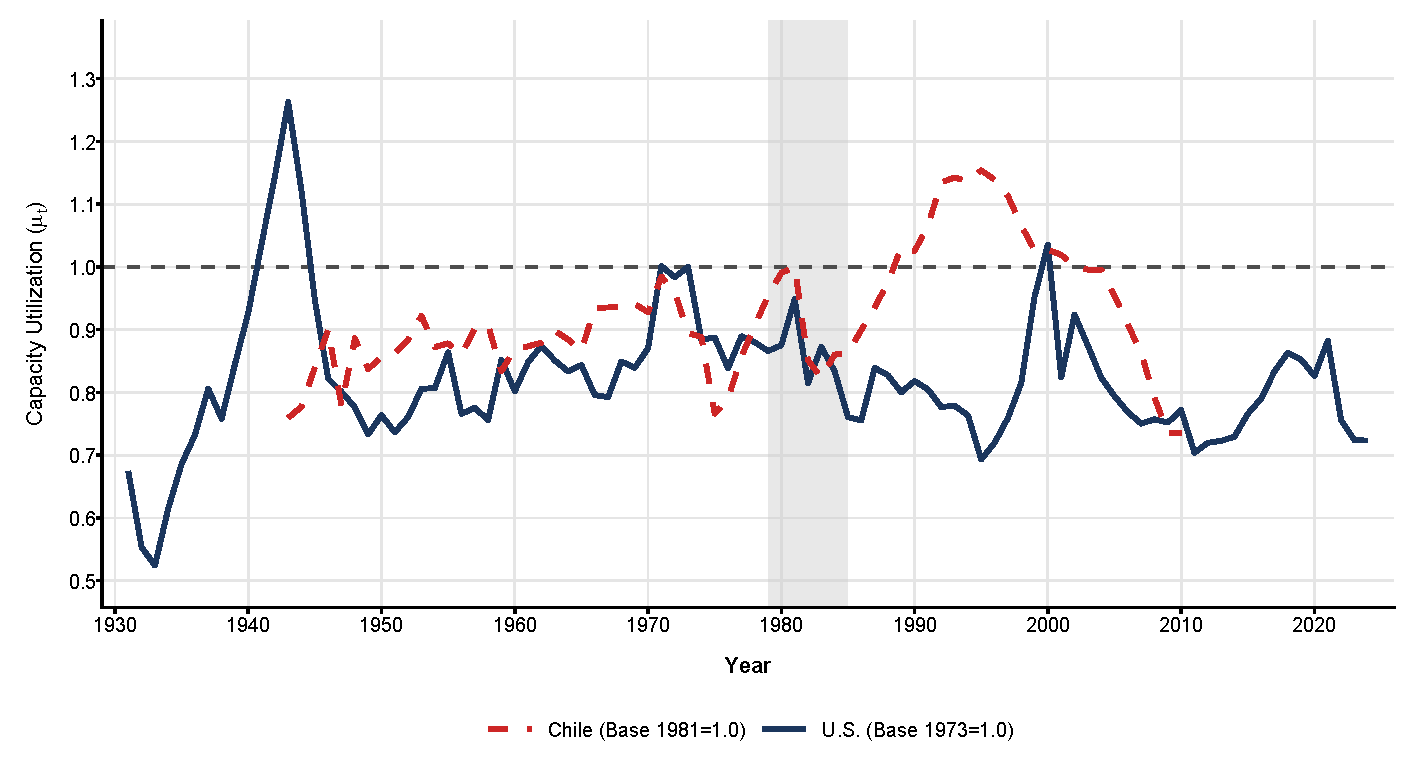
\includegraphics[width=\textwidth]{figures/fig_sec5_combined_mu.pdf}
	\begin{tabular}{p{0.92\textwidth}}
		\scriptsize \textbf{Note:} Implicit capacity utilization ($\mu_t$) for the U.S. (solid navy) and Chile (dashed crimson). The shaded band highlights the early 1980s global overaccumulation crisis (1979--1985), resolved via financialization in the center and external subordination in the periphery. \\
	\end{tabular}
\end{figure}

Neither economy in Figure~\ref{fig:sec5_combined_mu} converges toward a normal rate of utilization in the long run ($\mu = 100\%$); persistent idle capacity remains the structural norm of decentralized accumulation. The volatility of $\mu_t$ in Chile vastly exceeds that of the United States. This higher amplitude tracks the structural asymmetry between a diversified, reserve-currency center capable of dampening demand swings and a dependent periphery vulnerable to sudden international liquidity collapses; it is not an econometric anomaly. Installed gross fixed capital ($K_t$) cannot vanish during downturns, so peripheral output collapses, such as the supply shocks of 1975 and the 1982 debt crisis, translate into abrupt contractions of utilization. The shaded window (1979--1985) captures a global overaccumulation crisis and structural turning point: the Volcker interest-rate shock triggered a severe domestic realization drop in the center ($\mu_{1982} \approx 82\%$) while ending Chile's debt-led boom ($\mu_{1981} = 100\%$) and driving peripheral utilization into a macroeconomic trough. This common conjuncture was subsequently resolved through divergent regime shifts: debt-led financialization in the center, and a violent transition toward neoliberalization and external subordination in the periphery.

\paragraph{The Center: Realization Failure and Intellectual Monopolies.} 
In the United States, the dynamics of $\mu_t$ are governed by the continuous mediation of distributive conflict and the shifting composition of capital. Because capital goods are produced domestically, the transformation of accumulation into capacity ($\theta$) is not externally constrained; while stagnation and crisis may have multifaceted causes, they ultimately manifest as an issue of \textit{realization}. Under Atlantic Fordism, the institutionalized class compromise absorbed growing productive capacity via mass consumption \citep{Aglietta2000}. High wage shares, alongside negligible diversion of investment toward intangible assets like intellectual property, meant that consumer demand effectively matched expanding physical capacities, sustaining $\mu_t$ within a high, stable corridor (85--105\%). While a commitment to full employment, Keynesian policymaking, and demand-inducing militarism masked secular overaccumulation tendencies, distributive conflict exerted cost-minimizing pressures that forced capitalists to engage in mechanization, configuring a contradictory utilization regime. 

When the profit squeeze emerged in the late 1960s, $\mu_t$ fell to 76.2\% in 1975 and bottomed at 74.1\% in 1982 during the Volcker disinflation. In his decomposition of this postwar U.S. profit rate collapse, \citet{Weisskopf1979} pinned the crisis on the ``Rising Strength of Labor'' (RSL), treating the ``Realization Failure'' (RF) variant—a drop in $\mu_t$—as a secondary, survey-driven symptom. The Federal Reserve Board utilization series does not identify the physical conversion of accumulation into capacity. Here, $\mu_t$ is instead recovered as an endogenous residual of $\theta_t$. The Fordist profit squeeze was not just a distributional fight over a fixed pie; it was a structural breakdown in $\theta_t$ itself. When effective wage pressure peaked, $\theta_t$ fell to 0.32. The subsequent fall in $\mu_t$ directly reflected that distributive conflict degrading the capacity-generating power of capital. Post-Fordism dismantled the institutional foundations of wage-led growth to resolve this crisis. The capitalist class restored profitability through deunionization and wage suppression. This structural wage suppression nevertheless fundamentally undermined the domestic realization of productive capacity over the long run, an effect only partially offset by debt-led consumption \citep{Stockhammer2012,Vidal2019}. Average utilization failed to return permanently to its Fordist peaks, exceeding the 100\% benchmark temporarily only during the speculative tech-investment bubble of 2000 ($\mu_{2000} \approx 103\%$). Persistent idle capacity therefore accompanies the post-Fordist shift toward financialization and the growing weight of intangible-asset accumulation \citep{Rikap2021, Rotta2018}.

\paragraph{The Periphery: Dual Strangulation and Export Reprimarization.} 
The terminal crisis of the inward-oriented regime in the peripheral Chilean economy cannot be explained by the balance-of-payments constraint alone, nor by the domestic profit squeeze in isolation. As \citet{Prebisch1981} fundamentally articulated, the structural condition of the periphery is defined by its subordinate integration into the global division of labor. Because technological development inherently necessitates imported capital goods ($K^{\text{ME}}$) for late-industrializing economies, peripheral capitalist formations face a rigid structural ceiling: the transformation of accumulation into productive capacity is perpetually subject to the limits of external constraints. However, this external constraint did not operate in a distributive vacuum. Historical analyses of the Chilean developmental state emphasize that early import-substitution industrialization (ISI) was subsidized by a massive rural-to-urban demographic transition, providing an elastic urban reserve army \textit{\`a la} \citet{Lewis1954} that depressed real wages and temporarily offset chronic foreign exchange shortages \citep{Polanco2021}. Yet, as this rural surplus was exhausted by the late 1950s, the structural limits of the ISI model were exposed. The urban working class consolidated and distributive conflict intensified, culminating in the aggressive, wage-led redistribution of the \textit{Unidad Popular} (1970--1973).

In a closed economy, the 20-percentage-point rise in the gross wage share---from roughly 49\% in 1970 to a historical peak of 69.03\% in 1972---would have simply induced rapid labor-saving mechanization. In peripheral capitalism, however, the internal profit squeeze and the external balance-of-payments constraint locked together. The threshold cointegrating model formalizes why this distributive impulse failed to induce mechanization: as it rose, the composite balance-of-payments index fell deep into the binding domain ($Z_t = -1.06 < \hat{\gamma} = 0.425$). The external constraint truncated the choice of technique: peripheral capitalists retained the microeconomic incentive to substitute machinery for labor but lost the macroeconomic means. The working class's success in capturing a larger share of the surplus increased import demand for wage-goods, leaving insufficient foreign exchange to import capital goods. The cost of this ``dual strangulation'' appears in capacity utilization. When the \textit{Unidad Popular} assumed power, $\mu_t$ operated at a constrained baseline of 94.1\% in 1969. The initial redistributive boom drove $\mu_t$ to an unsustainable cyclical peak of 98.4\% in 1971. Deprived of the foreign exchange required to import machinery---exacerbated by credit blockades, capital flight, and the 1972 bosses' lockout \citep{DeVylder1976}---the economy lost more than 26 percentage points of utilization in just four years, reaching roughly 72\% by 1975. The unconverted distributive surplus manifested as a blocked surplus, generating structural inflation and severe supply bottlenecks rather than expanding productive capacity. 

The post-1975 resolution did not rebuild domestic manufacturing. While the unconstrained international liquidity conditions and copper booms of the 1990s temporarily pushed utilization to hyper-capacity levels ($\mu > 110\%$ during the 1993--1996 peak), leading to overheating and the Asian Crisis during the 1997-1998 period. In the aftermath, trade liberalization and financial opening ultimately locked the accumulation regime into premature de-industrialization and export reprimarization \citep{Palma2019}. Under the 2000s commodity super-cycle, external solvency was stabilized through primary extractive rents rather than domestic industrial capacity \citep{Torres2022, Ahumada2026}; high import leakages and multinational profit repatriation once again depressed capacity utilization to roughly 73\% by 2010. From an institutional design standpoint, this trajectory yields a critical lesson: redistributive programs in the periphery cannot succeed in isolation from strategic foreign-exchange regime and monetary policy articulated with effective cross-borders of capital controls \citep{Ffrench2018}. 

The composite index $Z_t$ and the threshold $\hat{\gamma} = 0.425$ are estimated via a deterministic hard classification. This binary gate captures the frequency with which the constraint binds, not smooth, probabilistic regime shifts. It captures the ``stop-go'' shocks of the ISI era and the intra-cycle tightness of the 2000s mining boom rather than positing a single macro-historical break, but does not provide granular identification within regimes. Within these limits, the classification captures the discrete severing of the transformation of accumulation into capacity whenever external solvency collapses in the periphery. Future research requires backward and forward extension of time-series and exploration of other econometric techniques, such as Markov-switching modelling, to assign a time-varying threshold for regime classification. Applying this double-constraint metric to comparative panel datasets across other commodity-dependent or semi-peripheral spaces remains a promising avenue for future research.

\paragraph{Synthesis: Dead Labour Across the Global Divide.}
This comparative analysis demonstrates that the contemporary political economy of capacity utilization is fundamentally dictated by an economy's position within the global division of labor as originally formulated by \citet{Prebisch1981}. In the current stage of \textit{"geriatric capitalism"} \citep{Vidal2019}, chronic idle capacity is not a mere anomaly, but the structural manifestation of overlapping stagnationist tendencies across the uneven development of the capitalist world system. In the center, this takes the form of an exhausted accumulation regime prone to secular stagnation: unable to mobilize idle physical capacity through wage-led demand, partially offset through debt-led consumption and later diverted to asset inflation and accumulation of intangible unproductive assets \citep{Rotta2018, Rikap2021}. In the periphery, the condition of financial subordination express through differential channels and the specific integration to the world market but with a common ceiling imposed by external constraints, insofar this become binding due financial imbalanced caused by a low degree of import capacities with respect to the effective demand for imports from domestic markets \citep{McCombieThirwall1994}.

The dead labour embedded in under-utilized productive capacities is crystallized past labour denied the living labour necessary for its valorization. In the center, this idleness accompanies the dismantling of a domestic social settlement in the name of profitability and financialized rent extraction; in the periphery, it reflects an asymmetrical global order that conditions growth on structural subordination. In both cases, accumulated capital remains physically present while the conditions for its reproduction are impaired.